\documentclass{article}
\usepackage{pgf}
\usepackage{tikz}
\usetikzlibrary{arrows,automata}
\usepackage[latin1]{}
\usepackage{fancyhdr}
\pagestyle{fancy}
\fancyhf{}
\rhead{ssamal@cse.unl.edu}
\lhead{CSCE828-Project1-DFA33}
\lfoot{\copyright Suraj Samal}
\rfoot{\thepage}
\begin{document}
\title{CSCE828-Project1-ssamal@cse.unl.edu}
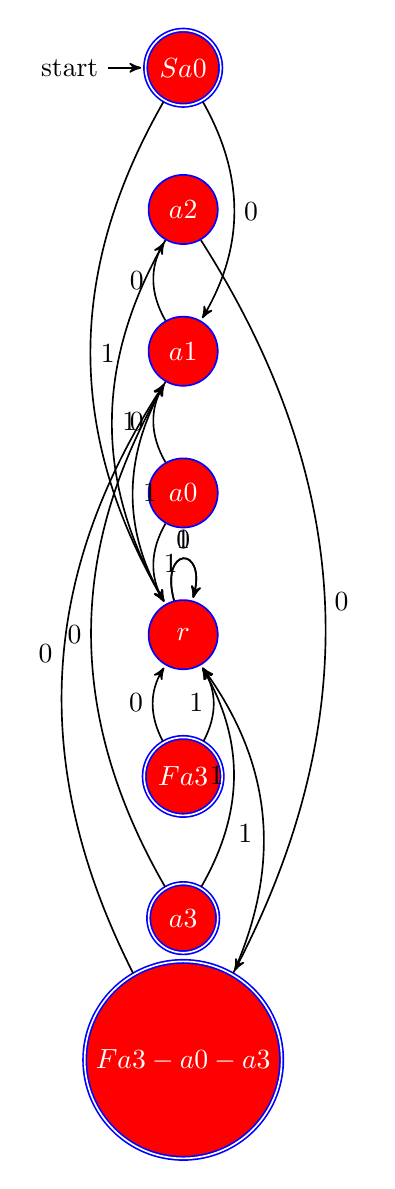
\begin{tikzpicture}[->,>=stealth',shorten >=1pt,auto,node distance=1.8cm,semithick]
   \tikzstyle{every state}=[fill=red,draw=blue,text=white]
   \node[state,initial,accepting]   (Sa0)        {$Sa0$};
   \node[state]   (a2)  [below of=Sa0]  {$a2$};
   \node[state]   (a1)  [below of=a2]  {$a1$};
   \node[state]   (a0)  [below of=a1]  {$a0$};
   \node[state]   (r)  [below of=a0]  {$r$};
   \node[state,accepting]   (Fa3)  [below of=r]  {$Fa3$};
   \node[state,accepting]   (a3)  [below of=Fa3]  {$a3$};
   \node[state,accepting]   (Fa3-a0-a3)  [below of=a3]  {$Fa3-a0-a3$};

   \path  
     (a2)  edge  [bend left]    node {0}  (Fa3-a0-a3)
     (a2)  edge  [bend right]    node {1}  (r)
     (Fa3)  edge  [bend left]    node {0}  (r)
     (Fa3)  edge  [bend right]    node {1}  (r)
     (a1)  edge  [bend left]    node {0}  (a2)
     (a1)  edge  [bend right]    node {1}  (r)
     (a3)  edge  [bend left]    node {0}  (a1)
     (a3)  edge  [bend right]    node {1}  (r)
     (Fa3-a0-a3)  edge  [bend left]    node {0}  (a1)
     (Fa3-a0-a3)  edge  [bend right]    node {1}  (r)
     (a0)  edge  [bend left]    node {0}  (a1)
     (a0)  edge  [bend right]    node {1}  (r)
     (Sa0)  edge  [bend left]    node {0}  (a1)
     (Sa0)  edge  [bend right]    node {1}  (r)
     (r)  edge  [loop above]  node {0}  (r)
     (r)  edge  [loop above]  node {1}  (r);
\end{tikzpicture}
\end{document}